\chapter{\IfLanguageName{dutch}{Proof of concept}{State of the art}}%
\label{ch:proof-of-concept}

Dit deel van het onderzoek stelt een Proof of Concept voor die zich richt op het web scrapen van het netwerkverkeer van een website zodat de gestructureerde data die verstuurd wordt van de server kan onderschept worden. Sommige van deze bestanden die de server verstuurd, bevatten de gestructureerde data die de website gebruikt om zijn inhoud dynamisch te genereren. In deze gestructureerde data is vaak meer informatie te vinden dan op de website getoond wordt. Dit zorgt voor een verhoogde kwaliteit van verzamelde data. Het vergt ook minder rekenkracht van de machine dat de web scraper op uitgevoerd wordt omdat de HTML-code niet geparsed hoeft te worden. De Proof of Concept bestaat uit een Python script.

\section{Vereisten}
Het uitvoeren van deze Proof of Concept vereist bepaalde software op het systeem. De vereiste software zijn:
\begin{itemize}
    \item Python \footnote{\url{https://www.python.org/downloads/}}
    \item De package manager pip~\footnote{\url{https://pip.pypa.io/en/stable/installation/}}
\end{itemize}

\section{Versies}
In deze Proof of Concept wordt gebruik gemaakt van Python versie 3.10.2. De python-Bibliotheken die in deze Proof of Concept gebruikt zullen worden zijn:

\begin{itemize}
    \item \textbf{json: } Deze Python-bibliotheek wordt gebruikt om met JSON-bestanden te werken. json is standaard geinstalleerd in Python

    \item \textbf{Requests: } Deze Python-bibliotheek wordt gebruikt om HTTP-verzoeken te maken.

    \item \textbf{Selenium: } Selenium wordt gebruikt om het netwerkverkeer op te halen.
\end{itemize}

Om mogelijke conflicten tussen de gebruikte Python-bibliotheken te voorkomen wordt gebruik gemaakt van een virtuele Python omgeving. Om de virtuele omgeving te creëren moet het commando \ref{cmd:createvenv} uitgevoerd worden.

\begin{lstlisting}[language=bash, label={cmd:createvenv}, caption={Het commando om een virtuele Python omgeving te creëren}]
    python -m venv /path/to/new/virtual/environment/
\end{lstlisting}
Om de virtuele Python omgeving te activeren op een Windows machine moet het commando \ref{cmd:startvenv} uitgevoerd worden, voor een moet het commando \ref{bash:startvenv} gebruikt worden.
\begin{lstlisting}[language=bash, label={cmd:startvenv}, caption={Het commando om een virtuele Python omgeving te activeren op een Windows machine}]
    venv\Scripts\activate.bat
\end{lstlisting}

\begin{lstlisting}[language=bash, label={bash:startvenv}, caption={Het commando om een virtuele Python omgeving te activeren op een Linux of MacOS machine}]
    $ source myvenv/bin/activate
\end{lstlisting}

Om de gebruikte Python-bibliotheken te installeren moet het commando \ref{cmd:req.txt} uitgevoerd worden. het bestand \texttt{requirements.txt} is te vinden op de github-pagina \footnote{\url{https://github.com/hannesroegiers/bachelorproef/tree/main/PoC}}van deze Proof of Concept. Dit bestand bevat de nodige Python-bibliotheken met de gebruikte versie.
\begin{lstlisting}[language=bash, label={cmd:req.txt}, caption={Het commando om de nodige Python-bibliotheken te installeren}]
    pip install -r requirements.txt
\end{lstlisting}

\section{Verkenning}
Op de doel website\footnote{\url{https://www.oddsportal.com/football/belgium/jupiler-pro-league/}} zijn een aantal voetbal wedstrijden te zien. Naast iedere wedstrijd staan 3 kolommen zoals te zien in \ref{fig:website1}. De cijfers die in deze kolommen staan zijn de data die de scraper gaat proberen te extraheren.

\begin{figure}[h]
    \centering
    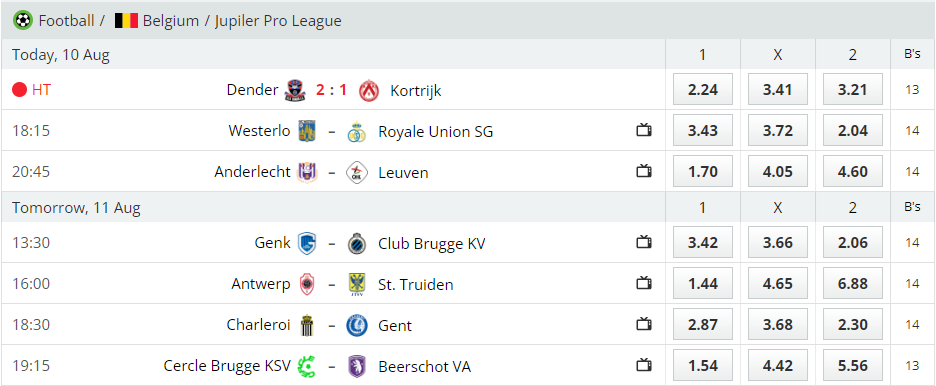
\includegraphics[width=\linewidth]{graphics/website1.png}
    \caption{De doel website}
    \label{fig:website1}
\end{figure}

\section{Analyse}
In deze tweede fase wordt er gebruikgemaakt van de Chrome browser en de developer tools binnenin Chrome. De developer tools kunnen geopend worden door op de functie toets \texttt{F12} te drukken of een klik op de rechtermuisknop te doen op de website en daarna op \texttt{Inspect} of \texttt{Inspecteren} te klikken. Wanneer deze website geladen wordt, stuurt deze een aantal HTTP-verzoeken naar de server. De antwoorden van deze verzoeken worden gebruikt om de inhoud van de website dynamisch op te bouwen. Deze HTTP-verzoeken en hun antwoorden zijn terug te vinden in het \texttt{Network} tabblad van de developer tools en stellen het netwerkverkeer van de website voor.

Voor web scrapen zijn er dus twee tabbladen in de developer tools die interessant zijn. Het \texttt{Elements} en het \texttt{Network} tabblad. Bij \texttt{Elements} kan de HTML-code -en structuur bekeken worden en in het \texttt{Network} tabblad kan het netwerkverkeer van de website bekeken worden zoals te zien in figuur~\ref{fig:networktab}. 

\begin{figure}[h]
    \centering
    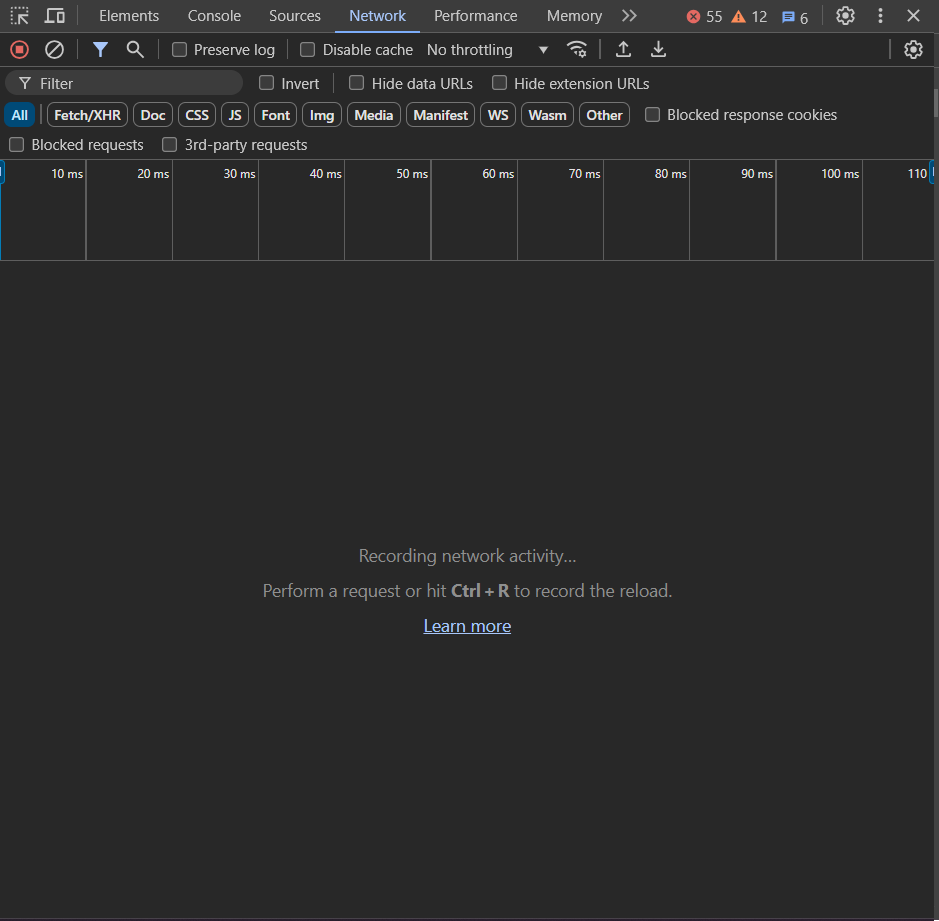
\includegraphics[width=\linewidth]{graphics/DevTools1.png}
    \caption{De developer tools, het netwerk tabblad}
    \label{fig:networktab}
\end{figure}

Wanneer de pagina herladen wordt, is in dit tabblad al het netwerkverkeer te zien dat tussen de client (website) en de server loopt~\ref{fig:networktab2}.

\begin{figure}[ht]
    \centering
    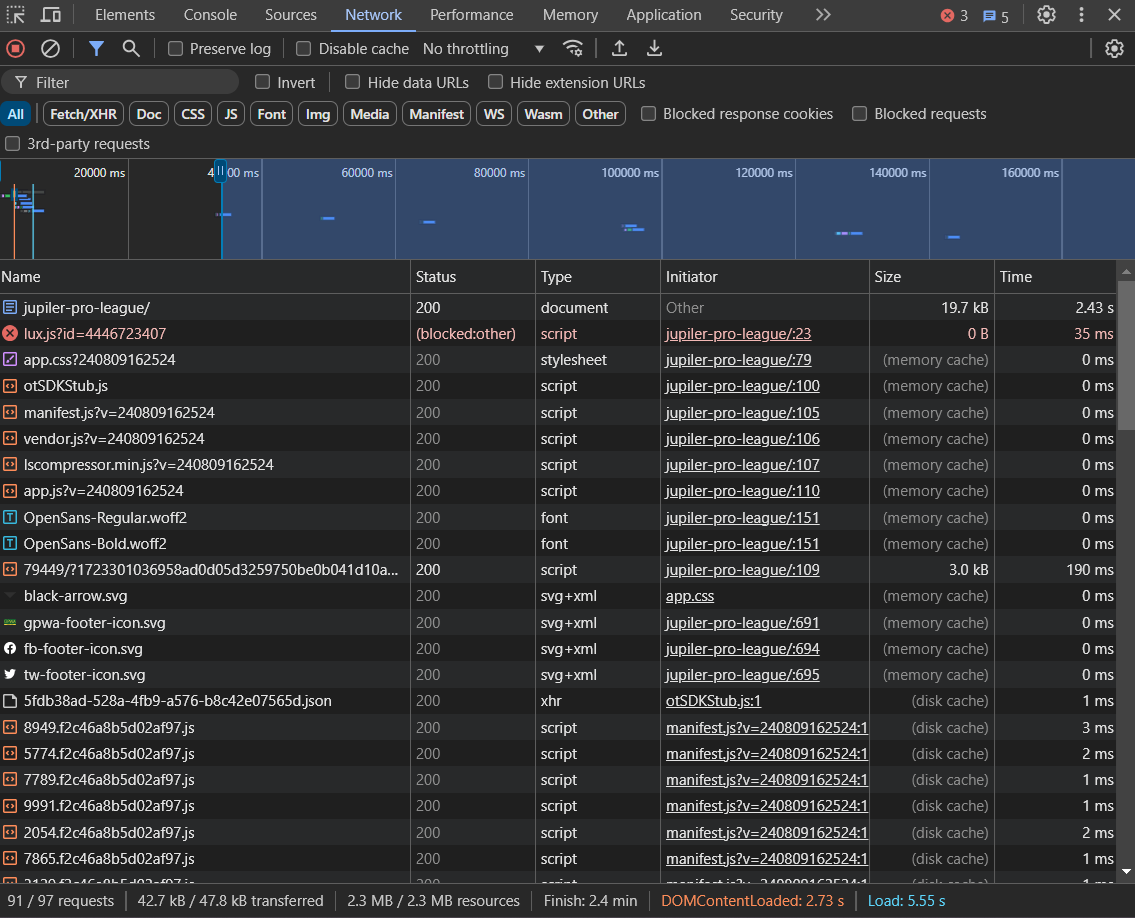
\includegraphics[width=\linewidth]{graphics/DevTools2.png}
    \caption{Het netwerkverkeer in de developer tools}
    \label{fig:networktab2}
\end{figure}

Hier zijn veel bestanden te vinden maar dit onderzoek richt zich op bestanden die gestructureerde data bevatten. In de developer tools kan hier op gefilterd worden door \texttt{Fetch/XHR} te selecteren. De meeste zichtbare bestanden zullen nu JSON en XML bestanden zijn.
